\documentclass[10pt, conference]{IEEEtran}
\IEEEoverridecommandlockouts

\usepackage{graphicx}
\usepackage{setspace}
\usepackage{wrapfig}
\usepackage{amsmath}
\usepackage{changepage}

\begin{document}

\title{Co-located and distributed MISO techniques in DVB-T2 Single Frequency Networks}

\author{
    \IEEEauthorblockN{Abdoul-Waris Gbadamassi}
    \IEEEauthorblockA{
        \textit{LETIA (of Polytechnic School of Abomey-Calavi) }\\
        \textit{University of Abomey-Calavi} \\
        Calavi, Benin \\
        Email: abdoulwarisgbadamassi@gmail.com
    }
    \and
    \IEEEauthorblockN{Anne-Carole Hontoga}
    \IEEEauthorblockA{
        \textit{Electromagnetism and Telecommunications Department}\\
        \textit{University of Mons} \\
        Mons, Belgium \\
        Email: anne-carole.hontoga@umons.ac.be
    }
    \and
        \IEEEauthorblockN{Véronique Moeyaert}
        \IEEEauthorblockA{
            \textit{Electromagnetism and Telecommunications Department} \\
            \textit{University of Mons} \\
            Mons, Belgium \\
            Email: veronique.moeyaert@umons.ac.be
    }
    \and
        \IEEEauthorblockN{Michel Dossou}
        \IEEEauthorblockA{
            \textit{LETIA (of Polytechnic School of Abomey-Calavi) }\\
            \textit{University of Abomey-Calavi} \\
            Calavi, Benin \\
            Email: michel.dossou@epac.uac.bj
    }
}

\maketitle

\begin{abstract}
% \onehalfspacing 
In this paper, the impact of various diversity schemes of Alamouti Multiple Input Single Output (MISO) technique applied in Digital Video Broadcasting-Terrestrial second generation (DVB-T2) system has been evaluated. The advantages of diversity technique in both co-located MISO and distributed MISO configurations are foreseen to apply in SFN robustness in a Single Frequency Network (SFN). Co-located and distributed techniques are the approaches for applying MISO in DVB-T2 system. While the former suggests that transmitters are installed in the same site, the latter proposes they are separated at distinct locations. The system performance is influenced by the highest Layer Signal Point (LSP) reception rate, the Signal to Noise Ratio (SNR) leading to a better performance, adapted to the Bit Error Rate (BER) criteria. Consequently, the Modulation Error Rate (MER) was used. The results have shown that co-located MISO technique outperforms SFN robustness by mitigating frequency selective fading with a lower BER in the SFN system. The MER value using co-located MISO technique outperforms distributed technique by 2.5 dB at 15.2 dB of BER=0.1\%. Furthermore, the MER values confirm the betterment of robustness of DVB-T2 system when distributed MISO is exploited.
\end{abstract}

\normalsize{
\textbf{\textit{Index Terms}—DVB-T2, co-located MISO, distributed MISO,
SFN}
}

\section{Introduction}
\linespread{1.2}
\normalsize{
The advance of digital technologies has introduced new
ways to access to multimedia or audiovisual content with
high bit rate transmissions. DVB-T2 is the second generation terrestrial broadcasting system which has been developed and published by European Telecommunications Standards Institute (ETSI) to deal with the first generation DVB-T shortcomings. Both DVB-T and DVB-T2 have exploited SFN for the purpose of spectrum efficiency, but they differently experiment the SFN impact. Multifrequency Network (MFN) transmitters deliver the same content using different frequencies whereas SFN transmitters transmit the same content using the same carrier frequency. However, the channel resulting from SFN \\exploitation can have deep cuts and spatial diversity technique is used in DVB-T2 to eliminate these deep notches \cite{1}, \cite{2}. }

\linespread{0.98}
\normalsize{
\indent During the last decade, DVB-T2 has been the object of many studies around the world with the purpose to give technical information to broadcasters about the deployment and further improve its performance. This standard is based on a system which includes many advanced techniques such as a robust Forward Error Correction (FEC) (Bose–Chaudhuri–Hocquenghem codes (BCH) and Low Density Parity Check (LDPC)), the rotated constellation technique and the MISO technique. The last two techniques are optional. However, they induce a high gain when they are used in this system. While the former is based on frequency diversity technique, the latter is based on spatial diversity technique. MISO technique has been mainly studied in the scientific literature to highlight its performance jointly with rotated constellation technique. Some works present MISO
performance in simulation using rotated constellation with
iterative demapper \cite{3}. Other works tackle SFN shortcomings by proposing an SFN with more than two transmitters, which allows spatial diversity technique to give good performance\cite{1}. However, to the best of our knowledge, no previous study has been done on comparison between distributed MISO and co-located MISO. The first uses transmitting antennas located at different sites whereas the second uses transmitting antennas located at the same site (Fig. 1). The advantage of co-located
MISO is that diversity gains are observed over the entire
coverage area, not just in overlapping areas as in distributed MISO. The advantage of distributed MISO is that no new radio equipment is required within the existing SFN, whereas co-located MISO requires duplication of transmitters \cite{4}. \\
\indent Indeed, as constellation rotation technique presents a better performance in presence of frequency selective channel but
in counterpart induces a high detection complexity, many
broadcasters do not exploit the benefit of this technique in the network. Furthermore, there is a gap within the performance gain comparison using MISO distributed and MISO co-located. This paper gives a compliant detail about MISO performance when rotated constellation is not applied. Performance are highlighted in the case of both co-located and distributed networks. Besides the BER used to evaluate system performance, MER is computed.
}

\begin{figure}[!htbp]
 \centering
    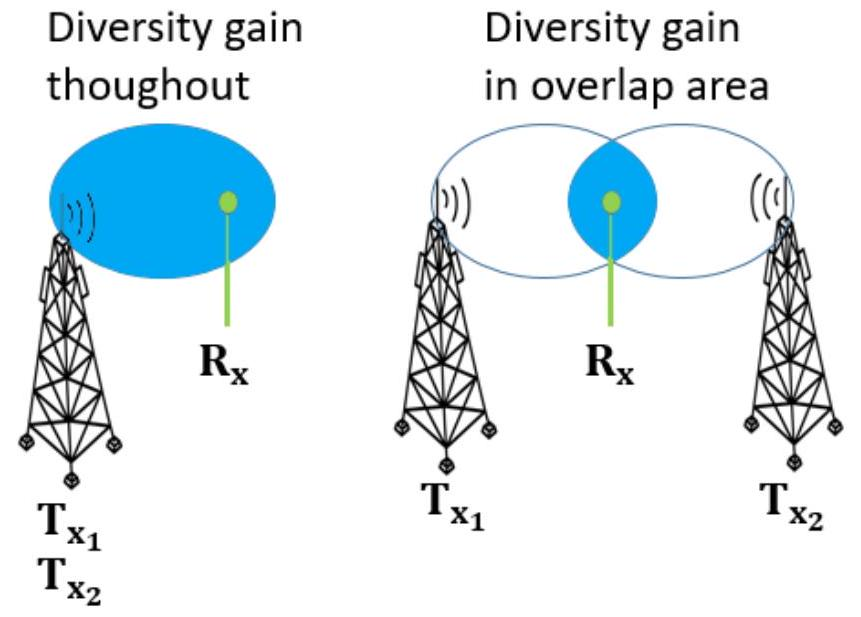
\includegraphics[width=0.47\textwidth]{images/img_1.jpg}
    \caption{Co-located MISO vs Distributed MISO.}
\end{figure}

\normalsize{
 \hspace{3em} 
 To achieve these goals, related works are presented (§II).
 This is followed by the spatial diversity technique (§III). Afterwards, the materials and methodology are presented (§IV). The simulation results and discussion are shown (§V). The paper is finalized by the conclusion (§VI).
}

\section{RELATED WORKS}    

\linespread{1.055}
\normalsize{
    \hspace{1em} This section provides an update on the various related works about DVB-T2 and MISO. In general, some works related to rotated constellation, SFN and MISO in DVB-T2 are discussed.
}

\normalsize{
    \hspace{1em} Comparison of the quality of radio coverage due to MFN based and SFN-based Digital Terrestrial Television Broadcasting (DTTB) system has been done \cite{5}. It has been showed that the high radio coverage resulted in the ‘SFN for maximum coverage’ is reasonably higher than compared to the coverage in the MFN.
}

\normalsize{
    \hspace{1em}  The impact of rotated constellation has been studied under 0 dB echo channel \cite{6} used to emulated SFN environment. The results have showed a very good performance of rotated constellation technique.
}

\normalsize{
    \hspace{1em} Based on measurement data, the rotation constellation effect has been evaluated in DVB-T2 \cite{7}. It is showed that the system that used the rotated constellation function have significant better results. However, this improvement comes at the cost of a higher complexity of the demodulation at the receiver side \cite{8}.
}

\normalsize{
    \hspace{1em} DVB-T2 and DVB-T systems performance have been compared in an SFN transmission \cite{1}. The results have showed DVB-T2 SNR performance improvement of 10 dB compared to DVB-T. This improvement allows reducing the transmission power compared to DVB-T transmission or to increase the coverage area in SFN
}
\linespread{0.95}
\normalsize{
    \hspace{1em} The advantages of MISO technique on a SFN DVB-T2 network have been identified [9]. It has been concluded that MISO technique allows improvements in the received SNR and also ensures that the ripples and notches do not occur in a SFN network. Only the distributed MISO was concerned.
}

\normalsize{
    \hspace{1em} Performance of MISO and SISO techniques have been compared in DVB-T2 system using a fixed reception scenario \cite{3}. It is showed that better performance are obtained with MISO technique when compared to the SISO one. MISO technique intends to reduce destructive interferences and improve the coverage of SFN. No distinction was made about different MISO-SFN topologies i.e., co-located and distributed.
}

\normalsize{
    \hspace{1em} Accurate measurement of echo power and echo delay in an SFN environment with OFDM technology, for both preechoes and post-echoes, has been done in SISO DVB-T SFN and MISO DVB-T2 SFN \cite{10}. The results have shown the diversity advantage using MISO technique in an SFN. Only distributed MISO case was investigated.
}


\normalsize{
    \hspace{1em} Performance of DVB-T2 using MISO with special fixed transmission scenarios have been studied. Results have shown that the transmission conditions have different influence on the overall MISO-based DVB-T2 system performance \cite{11}. Only DVB-T2 distributed SFN-MISO network has been only considered.
}

\normalsize{
    \hspace{1em} SFN effects have been analyzed, as well as the corresponding MISO gain margins for commercial and custom software defined radio (SDR) receiver implementations \cite{12}. The results showed that the MISO gain is restricted only to the overlapping areas of an SFN where a small power imbalance between MISO groups is present. It has been showed that degradation occurs in the non-overlapping regions of an SFN. Co-located MISO topology was not addressed and analysis is based on results before LDPC decoding.
}

\normalsize{
    \hspace{1em} The performances of different network combinations from the usage of MISO in an SFN for DVB-T2 have been evaluated and compared \cite{13}. It has been showed that the number of combinations depends on the number of transmitters. Also, the MISO gain depends on the organization and the position of antennas where some of them transmit the same symbols and others transmit modified symbols as defined by the DVBT2 implementation guidelines \cite{14} for Alamouti MISO. This study was focused on distributed MISO-SFN topology. The co-located MISO case was not addressed.
}

%wali

\section{\small Spatial Diversity Technique in DVB-T2}
\subsection{\small DVB-T2 System}
% PARTIE DE WALY------------------------------------------
\onehalfspacing
\normalsize{ DVB-T2 system includes five sub-systems such as coding and multiplexing sub-system, mode adaptation and stream adaptation sub-system, modulator sub-system, demodulator sub-system and stream decoder sub-system as shown in Fig. 2. The input of the system is Transport Streams (TS) and/or Generic Streams. This is managed by coding and multiplexing sub-system. This is a source coder. The Mode adaptation and Stream adaptation form the input processing module, which} 
\linespread{1.04} \normalsize{ generates a T2-MI (T2- Modulator Interface) stream. A T2-MI stream contains all the information about the T2-frames and their emitting time [14]. This stream contains a sequence of T2-MI packets, and each packet carries either Baseband frame or signalling information (L1 or SFN). The next step is to feed the modulator by a T2-MI stream. Based on the Baseband frames and T2-frame assembly instructions carried in the incoming T2-MI stream, the modulator produces DVB-T2 frames and emits them at the appropriate time for strict SFN synchronization. The modulator sub-system includes successively Bit Interleaver Coding and Modulation (BICM) block, MISO processing (optional), frame builder and Orthogonal Frequency Division Multiplexing (OFDM) generation blocks. BICM block in its turn contains FEC encoding, bit interleaver, bits to cells demultiplexer and Gray mapping (maps cells to constellation) blocks. In fact, OFDM generation block includes MISO processing, pilot insertion, Inverse Fast Fourier Transform (IFFT) processing, guard interval and P1 symbol insertion.}


\normalsize{
At the receiver side, the first component is the demodulator sub-system. This sub-system receives an RF signal from one or more transmitters (in an SFN case) in the network and outputs one transport stream. The following step is the Stream decoder sub-system, which receives the transport stream and outputs decoded video and audio. Figure 2 resumes DVB-T2 system.\\
The main sub-systems on which this work is focused are the modulator and the demodulator. MISO technique that rep
resents the technique which increases the system performance is presented in detail in the next subsection.
}

\begin{figure}[!htbp]
 \centering
    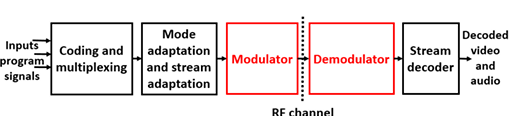
\includegraphics[width=0.45\textwidth]{images/2em_image.png}
    \caption{DVB-T2 system.}
\end{figure}

\subsection{Alamouti’s MISO}

\normalsize{
The idea of the MISO principle dates back to \cite{15} in
 1998 and is already used in mobile radio (LTE Long Term
 Evolution) where a repetition of adjacent symbols (COFDM
 symbols) at both two transmitting antennas is performed \cite{16}.
 At the receiving antenna, an overlapping grouping of adja
cent symbols is obtained which, without modification, would
 lead to mutual interference and make separation at reception
 impossible. MISO technique according to Alamouti also uses
 two transmitting antennas and one receiving antenna. The goal
 is to avoid the expenses related to receiver antenna by using
 transmission diversity also known as space-time diversity \cite{15}.
 On the other hand, for Alamouti’s MISO principle (according
 to Alamouti’s code (Fig. 3)), on the different transmitting
 antennas the adjacent symbols are transmitted with modifi
cation. The Alamouti code first stipulates the presence of
 the two adjacent symbols sn and sn+1 at antenna 1 and
 antenna 2 respectively. Then the symbol sn+1 is sent as a  negative conjugate complex through antenna 1 and at the
 same time the symbol sn is radiated as a conjugate complex
 through antenna 2. The receiver is thus able to separate
 the two adjacent symbols by means of appropriate complex
 mathematical operations on these symbols \cite{16}.
 MISO signal processing at reception is presented as follows :
 
 \begin{flushleft}
    Alamouti matrix: \hspace{2cm} received symbols:
\end{flushleft}

\[
\begin{array}{c cc}
    \text{time} & t_1 & t_2 \\ \hline
    \text{path}_1 & S_1 & -S_2^* \\
    \text{path}_2 & S_2 & S_1^* \\
\end{array}
\hspace{2cm}
\begin{array}{l}
    r_1 = S_1 + S_2 \quad (1) \\
    r_2 = -S_2^* + S_1^* \quad (2) \\
\end{array}
\]

    Combining rule in the receiver:
    
\begin{align}
    \tilde{S}_1 &= r_1 + r_2^* = (S_1 + S_2) + (-S_2^* + S_1^*)^* = S_1 + S_1 = 2 S_1 \\
    \tilde{S}_2 &= r_1 - r_2^* = (S_1 + S_2) - (-S_2^* + S_1^*)^* = S_2 + S_2 = 2 S_2 
\end{align}

 \begin{figure}[!htbp]
 \centering
    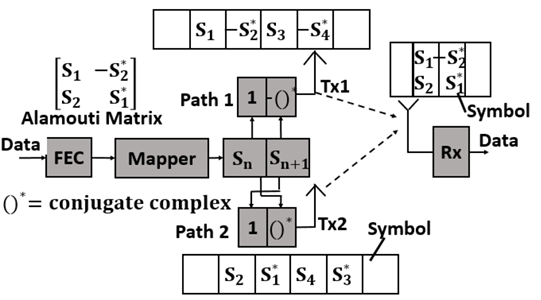
\includegraphics[width=0.45\textwidth]{images/3em_image.png}
    \caption{Principle of the MISO technique according to Alamouti (adapted from
 [16]).}
\end{figure}
}


\subsection{ Alamouti’s MISO adapted for DVB-T2}

\normalsize{
DVB-T2 uses a modified Alamouti coding (Fig 4). On
 antenna 1 the Quadrature Amplitude Modulation (QAM)
 symbols c1, c2, c3, c4,... which form the OFDM symbol
 are transmitted without change and on antenna 2 the corre
sponding modified symbols are transmitted. The advantage of
 this type of configuration is such that DVB-T2 system can
 be easily reduced to a SISO system by simply omitting the
 second antenna \cite{16}. Moreover, instead of using space/time
 diversity technique like presented in previous section (III.B)
 space/frequency diversity technique is used \cite{16}. Indeed, at
 the transmitting antenna 2 side, adjacent subcarriers pairs are
 exchanged with respect to those transmitted at transmitting
 antenna 1. The main advantage of this modified Alamouti
 principle is that the signals from transmitting antennas 1 and 2
 are no longer correlated with each other \cite{16}. This avoids the
 notches that are prevalent in DVB-T and DAB (Digital Audio
 Broadcasting), especially when using distributed MISO in a
 SFN \cite{16}.

}

 \begin{figure}[!htbp]
\centering
    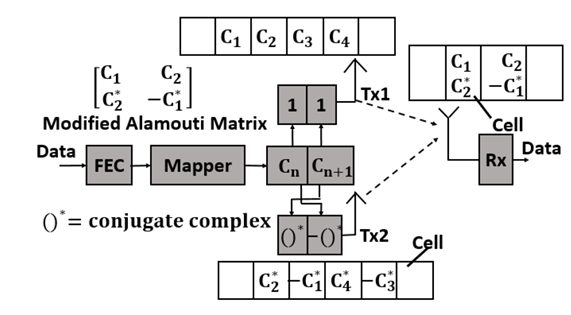
\includegraphics[width=0.45\textwidth]{images/4em_image.png}
    \caption{Principle of the MISO technique according to Alamouti (adapted from
 \cite{16}).}
\end{figure}

\linespread{1.055}

 \subsection{MATERIALS AND METHODOLOGY}
 
\subsubsection{Common Simulator Platform (CSP)\\} 

\normalsize{
The simulation of the DVB-T2 transmission system has
 been performed using the simulator CSP-DVB-T2. The CSP
 is a software implementation using MATLAB (Matrix Labo
ratory) of the DVB-T2 modulator, demodulator, and channel
 models. The software is constituted by three high-level direc
tories (“model”, “sim”, “utils”) [17] as shown in Fig. 5:}
\begin{itemize}
    \item \normalsize{“model” directory contains the end-to-end chain model
 including the transmitter, channel, and receiver. During a
 given simulation from the “sim” directory, functions of
 the model directory are called;} 

 \item \normalsize{ “sim” directory contains a number of different simula
tions. There are the “main” programs that invoke the
 model in a particular way and adapted to different applications.}
 \item \normalsize{ “utils” directory contains various utilities, including all
 the MATLAB scripts used to compare V\&V (Verification
 and Validation) files based on the DVB TM-T2 (DVB
 Technical Module T2) working group specifications, the
 L1 signaling decoding and display functions (provide the
 receiver with a means of accessing the physical layer
 pipes in T2 frames), and some bash scripts used to run
 the CSP and the comparison scripts.\\
 In reality, the “model” directory is the most important
 part of the CSP. However, the model directory is not very
 useful without the simulation (sim directory). The CSP
 is a good starting point, even if a user intends to develop
 his own simulator.
}

\begin{figure}[!htbp]
\centering
    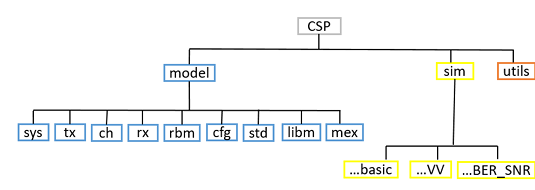
\includegraphics[width=0.48\textwidth]{images/5em_image.png}
    \caption{ Top-level directory structure (adapted from \cite{17}).}
\end{figure}
 
\end{itemize}

\linespread{1.8}
\subsubsection{System implemented}
\
The system is defined as the functional block of equipment
 performing the adaptation of the baseband TV signals from
 the output of the transport multiplexer to the characteristics
 of the terrestrial channel. The data stream is subject to the
 following processes at the transmitter side (Fig. 6) \cite{14}:
\begin{itemize}
    \item randomization for energy dispersion (scrambling);
    \item FEC coding (i.e., LDPC / BCH codes);
    \item bit interleaving;
    \item QAM modulation;
    \item frequency interleaving;
    \item IFFT and cyclic prefix insertion.
\end{itemize}
The emitted signal is subject to channel effects and the noise
 is adding. At the receiver side, the reverse operations of those
 performed at the transmitter side are performed.

\begin{figure}[!htbp]
 \centering
    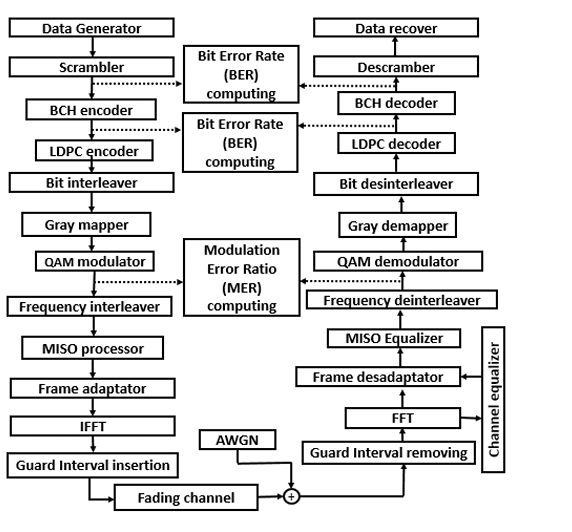
\includegraphics[width=0.488\textwidth]{images/6em_image.png}
    \caption{ System implemented.}
\end{figure}


\subsection{Channels}
\begin{itemize}
    \item \textbf{ Additve White Gaussian Noise (AWGN)}
\end{itemize}
\normalsize{ The signal from the transmitter to the receiver is always
 affected by noise. If there is no channel between the
 transmitter and the receiver, the received signal is only
 affected by a defined noise level. This channel is covered
 with AWGN, which is mainly produced in the receiver
 itself. The ideal condition for data reception is defined as
 a Gaussian channel \cite{18}.
 }




 
%elvis
%la suite d'une autre ligne
\linespread{1.15}
\normalsize{
\noindent Of Sight) which is added in F1 channel \cite{18}. In fact, P1 channel lets through only the delayed version of
the signal (20 delayed versions). Moreover, each delayed
path is associated with the attenuation, phase, and delay
values defined in the implementation guidelines \cite{14}.
The frequency responses of these channels are such that
they significantly attenuate the signal power at given
frequencies and maintain the power at other frequencies
[19]. To represent portable reception, the P1 channel is
used. The F1 channel represents a fixed reception.
\begin{adjustwidth}{-0.5cm}{0cm}
   \textbullet \textbf{ 0 dB echo channel}
\end{adjustwidth}
The 0 dB echo channel is an erasure channel with a
time profile that has two paths of equal amplitude [19].
The particularity of this channel lies in the fact that
the second path has a delay equivalent to 90% of the
duration of the guard interval with respect to the first
path \cite{19}. Also, the two paths are not attenuated. This is
the channel most often used to model SFN. It has been
proved that the reference 0 dB echo profile suggested by
the implementation guidelines \cite{14} seems to be optimistic
if used as reference SFN channel profile \cite{12}.

\begin{quotation}
    \begin{adjustwidth}{-2cm}{0cm}
        \begin{em}
            D. Performance analysis tools
        \end{em}
    \end{adjustwidth}
\end{quotation}
\begin{adjustwidth}{-0.5cm}{0cm}
   Two analysis tools have been used in this paper. These are
\end{adjustwidth}
\begin{adjustwidth}{-1cm}{0cm}
   the BER and the MER.
\end{adjustwidth}
\begin{adjustwidth}{-0.5cm}{0cm}
   \textbullet \textbf{  Bit Error Rat}
\end{adjustwidth}
BER is a quantitative criterion for analyzing the per-
formance of a digital link. The bit error rate is the
primary parameter describing the quality of the digital
transmission.

\begin{adjustwidth}{1cm}{0cm}

{\scriptsize 

\[
  BER = \frac{Number\hspace{0.5em}of\hspace{0.5em}erroneous\hspace{0.5em}bits}{Total\hspace{0.5em}number\hspace{0.5em}of\hspace{0.5em}bits\hspace{0.5em}transmitted}
  \hspace{2em} (5)
\]}
\end{adjustwidth}
It is defined as the ratio between the erroneous bits and the total number of bits transmitted, as show by equation
5.

\noindent Two methods are presented in the literature to calculate
the BER. The Monte-Carlo method which is based on
bits counting and requires a high computation time. The
second method is the EVM (Error Vector Magnitude)
which computes the analytic bit error rate. This method
is under the scope of this paper.

\begin{adjustwidth}{-0.5cm}{0cm}
   \textbullet \textbf{  Modulation Error Ratio}
\end{adjustwidth}
MER provides a unique analysis of the “quality factor”
of the received signal. This factor is calculated to include
the total signal degradation that may occur at the input
of the commercial receiver’s decision circuits. It provides
an indication of the ability of the receiver to decode the
signal correctly \cite{15}.

\noindent Let us consider M coordinate pair $(Ij, Qj)$ as ideal symbols. At the receiver side, we find N coordinate pairs
of the received symbols $(Ij + \delta Ij, Qj + \delta Qj)$. N must be
significantly  greater than the points
 of the M symbols. For
each received symbol, we check the transmitted symbol.
The error vector is defined as the distance between the ideal position of the chosen symbol and the actual
position of the received symbol. The difference can be
expressed as the vector $(dj = (\delta Ij, \delta Qj))$.

\begin{figure}[!htbp]
\centering
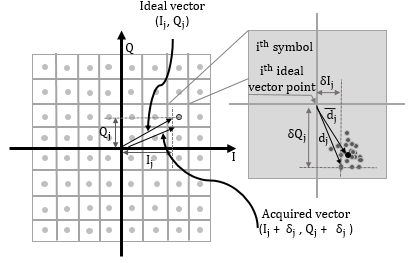
\includegraphics[width=8cm]{graph.png}
\begin{adjustwidth}{-0.13cm}{0cm}
\caption{\footnotesize Example of a constellation diagram for a 64-QAM modulation format, where the $i^{th}$ point has been enlarged to show the error vector coordinates of the symbols (adapted from \cite{20}).}
\end{adjustwidth}
\end{figure}

\noindent As shown in Fig. 7 for each symbol M, a cloud of error
vectors appears. The sum of the square of the magnitudes
of the vectors of the ideal symbols is divided by the sum
of the square of the magnitudes of the error vectors. The
result, expressed as the power ratio in dB, is defined as
the modulation error ratio.

\begin{adjustwidth}{0.5cm}{0cm}
\section*{ {\scriptsize  \textmd{V. SIMULATIONS RESULTS AND DISCUSSION}}}
\end{adjustwidth}

\begin{adjustwidth}{-0.13cm}{0cm}
 Table I shows the main settings which are used to simulate
DVB-T2 transmission over different channels in this paper.
These parameters are those which are the most used by the
DVB-T2 system implemented around the world \cite{20}.
\end{adjustwidth}

\begin{table}[!htbp]
\centering
{\small
\begin{center}
{\small TABLE I\\
SIMULATIONS PARAMETERS.}
\end{center}

\begin{tabular}{|l|r|}
\hline
Parameters & Values \\
\hline
Channel bandwidth & 8 MHz \\
\hline
FFT Mode & 32 K — Extended \\
\hline
Guard interval & 1/16 \\
\hline
Scattered pilot pattern & PP2 \\
\hline
LDPC size & 64800 \\
\hline
T2 frame length & 83 symbols \\
\hline
Number of T2 frame per super frame & 1 \\
\hline
Code rate & 2/3 \\
\hline
Constellation rotation & OFF \\

\hline
\end{tabular}
}
\end{table}

The objective of the MISO study is to highlight the per-
formance improvement which is achieved in an SFN. The
simulation methodology is summarized as follows:

1- Our system is validated by comparing the results obtained
with those presented in DVB-T2 guidelines in the presence of
AWGN. These results are used as reference afterwards.

2- Once the validation is done, DVB-T2 system is simulated
using F1, P1 and 0 dB echo channels (channels emulating an
SFN) in SISO technique.
}

\linespread{1.10}
\normalsize{
3- Afterwards the two most frequency selective channels
(P1 and 0 dB echo channels), are used to simulate an DVB-
T2 transmission with MISO technique both in co-located and
distributed cases.

It is relevant to note that for co-located SFN-MISO, the
implementation is done with four transmitter antennas where
two represent the direct paths and others are echos have
the same echo value $(0.9\Delta$ with $\Delta$ guard interval value). In
the case of distributed SFN-MISO, four transmitter antennas
have been used too. One represents direct path and three
others representing echos have respectively as echo values
$0.18\Delta$, $0.7\Delta$ and $0.9\Delta$. The direct path and one echo of
$0.9\Delta$represent the transmitter group 1 and transmit the same
symbols, and the two others representing the transmitter group
2 transmit the modified symbols. In addition, the Quasi Error-
Free (QEF) reception without rotation constellation \cite{14}, \cite{16}
is defined at BER after BCH decoding less or equal to $10^{-6}$ in
DVB-T2. So the chosen BER value is $10^{-5}$ for good analysis
purposes. In fact, all the curves reach at least this value.

\begin{adjustwidth}{0cm}{0cm}
    \textmd{ A. AWGN case}
\end{adjustwidth}

This subsection represents the first step of simulation
methodology. Fig. 8 and Fig. 9 show respectively the evolution
of BER and MER as a function of SNR for 64-QAM and
256-QAM constellations. The analysis of Fig. 8 shows a
decrease of BER with the evolution of SNR independently of
the constellation size. We conclude that as the signal power
becomes higher and higher compared to the noise power,
the BER decreases, i.e., improves. On the Fig. 9 the MER
increases with the increasing of the SNR. Moreover, this MER
is approximately equal to the SNR. We conclude that the more
the power of the signal compared to the noise increases, the
less we have errors in the constellation of the modulation
format and therefore the better the performance of the receive

\begin{figure}[!htbp]
\centering
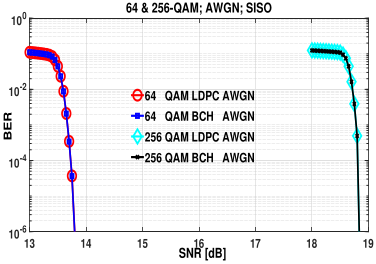
\includegraphics[width=7cm]{cap1.png}
\caption{
  \textup{{\footnotesize Evolution of BER as a function of SNR after LDPC and BCH decoding
for 64-QAM and 256-QAM constellation in the presence of AWGN.
}}}
\end{figure}

\begin{adjustwidth}{0cm}{0cm}
    \textmd{ B. Ricean case}
\end{adjustwidth}

This subsection takes into account the second step of sim-
ulation methodology. Fig. 10 and Fig. 11 show the simulation

\begin{figure}[!htbp]
\centering
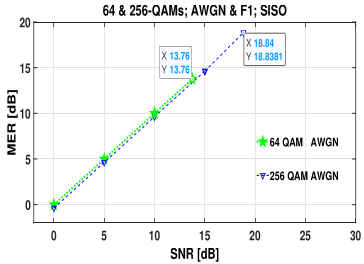
\includegraphics[width=7cm]{cap2.png}
\caption{
  \textup{{\small Evolution of MER as a function of SNR for 64-QAM and 256-QA constellation in the presence of AWGN.}}}
\end{figure}
  
\noindent results when Ricean fading channel is applied. On Fig. 10 a
little bigger SNR is required to achieve a BER of $10^{-5}$ after
BCH decoding when compared to SNR required for AWGN.

On Fig. 11 for a value of SNR required to achieve a BER
of $10^{-5}$ after BCH decoding, the corresponding MER value
whatever the constellation’s order is lower for Ricean fading
channel case than AWGN case.

\begin{figure}[!htbp]
\centering
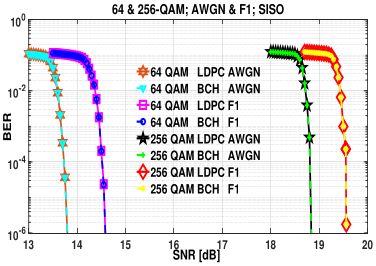
\includegraphics[width=7cm]{cap3.png}
\caption{
 \normalsize{Evolution of BER as a function of SNR after LDPC and BCH
decoding for 64-QAM and 256-QAM constellation for AWGN and F1 channel
with SISO technique.}}
\end{figure}



\begin{adjustwidth}{0cm}{0cm}
    \textmd{ C. Rayleigh case}
\end{adjustwidth}


In this subsection, we focus on the second and third steps
of simulation methodology. Fig. 12, Fig. 13 and Fig. 14
present respectively the BER and MER evolution in function
of SNR for SISO case and two MISO cases (co-located and
distributed) with P1 channel. In Fig. 12 and Fig. 13 we note a
higher SNR requirement for SISO case than co-located MISO
in order to achieve a BER of $10^{-5}$ after BCH decoding. The
distributed MISO case needs at its turn less SNR than this last
one for achieving the same goal.
}

 
%schekina

\begin{figure}[!htbp]
\centering
    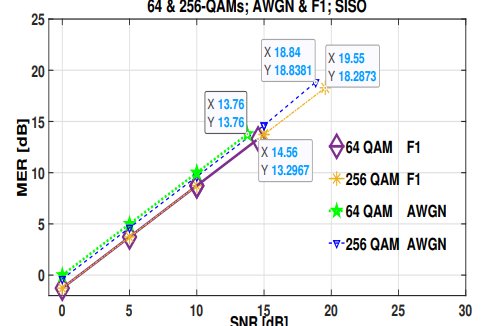
\includegraphics[width=8.5cm]{img1.png}
    \caption{ Evolution of MER as a function of SNR for 64-QAM and 256-QAM constellation with AWGN and F1 channel with SISO technique.}
\end{figure}
\linespread{1.1}
\normalsize{
In terms of MER values which correspond to required SNR which permit to reach a BER of $10^{-5}$ after BCH decoding (Fig. 14), the Rayleigh channel MER values for co-located MISO case whatever the constellation’s order are a little lower than those values for SISO. In this last one, MER values are less than distributed MISO values.


\begin{figure}[!htbp]
\centering
    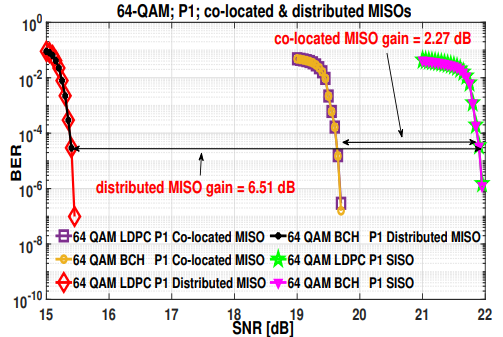
\includegraphics[width=8.5cm]{img2.png}
    \caption{Evolution of BER as a function of SNR after LDPC and BCH decoding for 64-QAM constellation for P1 channel with SISO, Co-located MISO and distributed MISO techniques.}
\end{figure}


 D. 0 dB Echo Case\\
Like the previous subsection, this subsection is also a part of the second and third steps of simulation methodology. Fig. 15, Fig. 16 and Fig. 17 present respectively the BER (Fig. 15 and Fig. 16) and MER (Fig. 17) evolution in function of SNR and the results are presented for the SISO case and two MISO cases (co-located and distributed) for 0 dB echo channel. The analysis of Fig. 15 and Fig. 16 shows a higher SNR requirement for SISO case than co-located MISO in order to achieve a BER of $10^{-5}$ after BCH decoding. The distributed MISO case needs at its turn less SNR than this last one.
}

\linespread{1}
\begin{figure}[!htbp]
\centering
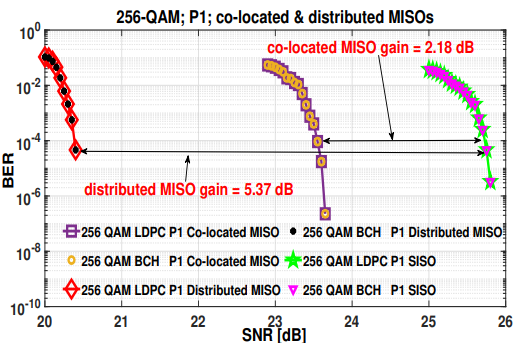
\includegraphics[width=8.5cm]{img3.png}
    \caption{ Evolution of BER as a function of SNR after LDPC and BCH decoding for 256-QAM constellation for P1 channel with SISO, Co-located MISO and distributed MISO techniques.}
\end{figure}

\begin{figure}[!htbp]
\centering
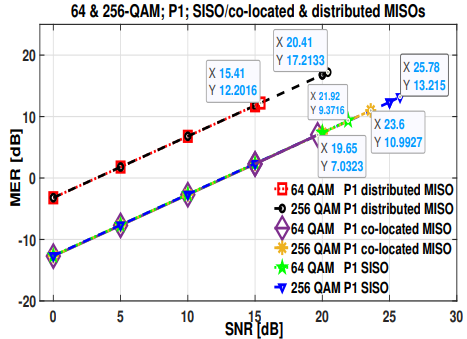
\includegraphics[width=8.5cm]{img4.png}
    \caption{Evolution of MER as a function of SNR before QAM demodulation for 64-QAM and 256-QAM constellation in the presence of P1 channel with SISO, Co-located MISO and distributed MISO techniques.}
\end{figure}

\normalsize{
for achieving the same goal. In terms of MER values which correspond to required SNR which permit to reach a BER of $10^{-5}$ after BCH decoding (Fig. 17), the 0 dB echo channel MER values for SISO case whatever the constellation’s order are a little lower than those values for distributed MISO. This last one MER values are lower than those co-located MISO values. 

Table II summarizes the different obtained MISO gains.

E. Discussion

In the absence of the rotated constellation technique, DVB-T2 standard provides a BER of $10^{-4}$ after LDPC decoding and $10^{-6}$after BCH decoding. The DVB-T2 system in the presence of additive white Gaussian noise only, without the constellation rotation technique, with a code rate of 2/3 for the LDPC encoder and a normal frame (64800 bits) has foreseen a signal-to-noise ratio specific to each constellation size. Thus, it is envisaged SNR of 3.1 dB, 8.9 dB, 13.6 dB,
}

\begin{figure}[!htbp]
\centering
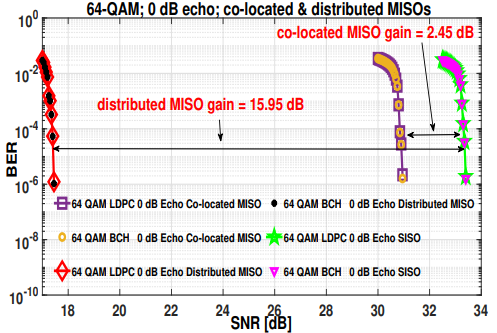
\includegraphics[width=8.5cm]{img5.png}
    \caption{Evolution of BER as a function of SNR after LDPC and BCH decoding for 64-QAM constellation for 0 dB echo channel.}
\end{figure}

\begin{figure}[!htbp]
\centering
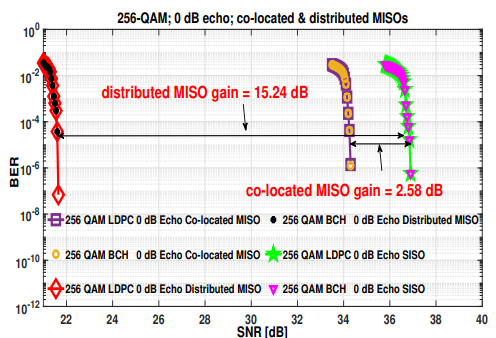
\includegraphics[width=8.5cm]{img6.png}
    \caption{Evolution of BER as a function of SNR after LDPC and BCH decoding for 256-QAM constellation for 0 dB echo channel.}
\end{figure}


\begin{figure}[!htbp]
\centering
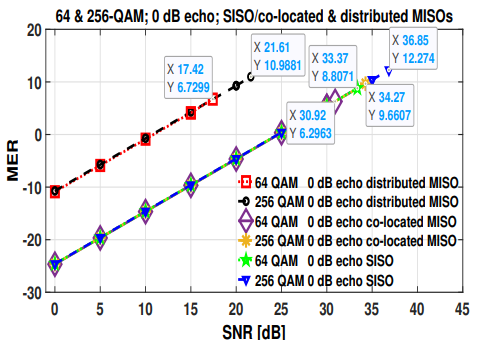
\includegraphics[width=8.5cm]{img7.png}
    \caption{Evolution of MER as a function of SNR before QAM demodulation for 64-QAM and 256-QAM constellation in the presence of 0 dB echo channel.}
\end{figure}


\begin{table}[!htbp]
\centering
\begin{center}
{\small TABLE I\\
SIMULATIONS PARAMETERS.}
\end{center}
\begin{tabular}{|p{1.7cm}|p{1.45cm}|p{1.96cm}|p{2.05cm}|}
\hline \footnotesize
Constellations & \footnotesize Channel & \footnotesize MISO topology & \footnotesize MISO Gains [dB] \\
\hline
64-QAM & P1 \par 0 dB echo & Colocated \par Distributed \par Colocated \par Distributed & 2.27 \par 6.51 \par 2.4 \par 15.95 \\
\hline
256-QAM & P1 \par 0 dB echo & Colocated \par Distributed \par Colocated \par Distributed & 2.18 \par 5.37 \par 2.58 \par 15.24 \\
\hline
\end{tabular}
\end{table}

\linespread{1.08}
\normalsize{
18.1 dB respectively for the constellations of order 4, 16, 64 and 256. Thus, there is an increasing need for higher SNR for good reception as the constellation size increases. We have focused on the high order constellations because they favor an increase in the transmission rate, and they are the most used in the different DVB-T2 systems around the world. Regarding the MER, it is expected that in the presence of AWGN only the SNR should be approximately equal to the MER. On the basis of these different performances provided by the standard, the simulator has been validated. With the increase of the constellation order, the performance degradation of the system in terms of SNR regresses. Regarding all the curves on Fig. 10 we can conclude that the minimum SNR value needed to have  good reception increases with the constellation order. Similarly, the performance degradation is higher in the presence of the Rayleigh and 0 dB echo channels. This is due to the high frequency selectivity of these two channels. This behavior confirms the impact of fading channel in DVB-T2 system.

The presence of chose channels in the DVB-T2 system leads to performance degradation in terms of MER (Fig. 11, Fig. 14 and Fig. 17) compared to the ideal case (AWGN only). This performance degradation evolves with the increase of the channel selectivity degree. But for each considered channel, the MER improves with the growth of the constellation order.

The insertion of the MISO technique in the system has led to an improvement in system performance in terms of SNR, which we call MISO gain, reaching 2.58 dB for colocated MISO and 15.24 dB for distributed MISO in a single frequency network for a high-order constellation equal to 256. This performance improvement which induces a decrease of the BER value has thus led to a decrease of the MER value linked to each constellation order at each channel. This is explained by the relationship between BER and MER, which states that a low BER value leads to a low MER \cite{3}.

When MISO technique is applied in the presence of frequency selective channels, the performance increase compared to those obtained in SISO case, at a BER of $10^{-5}$. In the Rayleigh case, a performance gain of 2.18 dB is achieved using MISO co-located topology. This performance increases up to 5.37 dB when the MISO distributed topology is used. In SFN environment case, the performance gains of 2.58 dB and 15.24 dB are obtained respectively for MISO colocated and distributed topologies. From all the foregoing, MISO distributed is the scheme which presents the better\\
%dernière page
performance. The higher improvement obtained with MISO distributed could be explainable by the presence of two other transmitters with a delay lower than that presented with the second transmitter in SISO. In other words, MISO performance increases with the number of transmitters used in SFN while maintaining the constraints of maximum distance between SFN transmitters. In perspective, the analysis of the MISO gain can be carried out analytically based on the work in \cite{1}.

\section{CONCLUSION}
In this paper, the impact of the MISO technique has been evaluated when the rotated constellation is not applied. It is proven that MISO with the distributed topology presents better performance in Rayleigh case and SFN environment. This work helps broadcasters optimize network coverage for DVB-T2 deployments.
}
\begin{thebibliography}{99}
\bibitem{1} M. Tormos, C. Tanougast, A. Dandache, D. Masse and P. Kasser, "Modeling and performance evaluations of Alamouti technique in a single frequency network for DVB-T2," \emph{EURASIP Journal on Wireless Communications and Networking}, pp.1-12, 2013.
\bibitem{2} EN 302 755 V1.4.1 (2015-07). Digital Video Broadcasting (DVB); Frame structure channel coding and modulation for a second-generation digital terrestrial television broadcasting system (3), European Standard ETSI, 2015.
\bibitem{3} L. Polàk, O. Kaller, and T. Kratochvil, "SISO/MISO Performances in DVB-T2 and Fixed TV Channels," \emph{38th International Conference on Telecommunications and Signal Processing (TSP)}, Prague, Czech Republic, July 2015.
\bibitem{4}J. L. Schadler, “ATSC 3.0 Boosting the Signal Strength – MISO,” BEIT
Proceedings, 2017.
\bibitem{5}S. Nepal et al., “A Comparative Study on Radio Coverage Due to DVB-T2 Multi-Frequency Network (MFN) and Single Frequency Network
(SFN)”, Proc.of Int. Symp. BMSB, pp. 1-6, 2020.
\bibitem{6}L. Polàk and T. Kratochvil, “Performance of the Rotated Constellation
in DVB-T2,” ICDT 2012 : The Seventh International Conference on
Digital Telecommunications, Mont Blanc, France, May 2012.
\bibitem{7}N. Suwansukho and S. Promwong, “Evaluation of Rotated Constellation
in DVB-T2 Based on Measurement Data,” 5th International Conference
on Engineering, Applied Sciences and Technology (ICEAST), Luang
Prabang, Laos, July 2019.
\bibitem{8}T. Kratochvil and R. Štukavec, “DVB-T Digital Terrestrial Television
Transmission over Fading Channels,” Radioengineering, vol.17, no. 3,
pp. 96-102, September 2008.
\bibitem{9} L. Andoni and A. Biberaj, “Multi-Antenna Systems in DVB-T2/SFN
Networks,” International Refereed Journal of Engineering and Science
(IRJES), ISSN (Online) 2319-183X, (Print) 2319-1821, vol.8, Issue 1,
PP. 66-70, January 2019.
\bibitem{10}G. Lu, X. Feng, J. Le and H. Zhang, “Single Frequency Network
measurement for digital video network,” IEEE International Symposium
on Broadband Multimedia Systems and Broadcasting (BMSB), Seoul,
Korea (South), June 2012.
\bibitem{11} L. Polak, J. Kufa, R. Sotner and T. Kratochvil, “On the Performance of
DVB-T2 MISO System: Special Fixed Transmission Scenarios,31st In-
ternational Conference Radioelektronika (RADIOELEKTRONIKA), pp.
1-4, April 2021.
\bibitem{12} J. Morgade, P. Angueira, A. Arrinda, R. Pfeffer, V. Steinmann, J. Frank,
and R. Brugger, “SFN-SISO and SFN-MISO Gain Performance Analysis
for DVB-T2 Network Planning,” IEEE Transactions on Broadcasting,
vol. 60, no. 2, pp. 272-286, 09 January 2014.
\bibitem{13} M. Tormos, C. Tanougas, P. Kasser, P. Bretillon and A. Dandache,
“Performance evaluation for different MISO-SFN network combinations
for DVB-T2 standard,” IEEE International Symposium on Broadband
Multimedia Systems and Broadcasting (BMSB), Nuremberg, Germany,
June 2011.
\bibitem{14} TS 102 831 V1.2.1 (2012-08). Digital Video Broadcasting (DVB),
Implementation guidelines for a second generation digital terrestrial
television broadcasting system (DVB-T2), ETSI Technical Specification,
2012.
\bibitem{15} M.S. Alamouti, “A Simple Transmit Diversity Technique for Wireless
Communications,” IEEE Journal on Selected Areas in Communications,
vol. 16, no. 8, pp. 1451-1458, Oct. 1998.
\bibitem{16} W. Fisher, “Signal and communication technology: Digital Video and
Audio Broadcasting Technology; A Practical Engineering Guide Book,”
in Springer, 4th ed., 1055 pages, 2020.
\bibitem{17} O. Haffenden, “DVB-T2 : The Common Simulation Platform,” Research
White Paper (WHP 196), British broadcasting corporation, May 2011.
\bibitem{18} L. Polàk and T. Kratochvil, “Analysis and simulation of the signals’
transmission in the DVB-H/SH standards,” Brno university of technology
: faculty of electrical engineering and communication departement of
radio electronics, doctoral thesis, 126 pages, 2012.
\bibitem{19}N. Cornillet, “Convergence des réseaux de télécommunications mobiles
et de télédiffusion : modélisation et évaluation des performances d’un
réseau hybride LTE/DVB-T2,” Université européenne de Bretagne,
thèse, 127 pages, dec.2013.
\bibitem{20} IUT-T, “J.142: Methods for the measurement of parameters in the
transmission of digital cable television signals,” 45 pages, 05/2000.
\bibitem{21} S. Jeon, J. Kim, H.-K. Mok, and J.-S. Seo, “Formulating the net gain
of MISO-SFN in the presence of self-interferences,” Radioengineering,
vol. 24, no. 2, pp. 643–649, June 2015
\end{thebibliography}
\end{document}
